
\documentclass{article}
\usepackage{listings}
\usepackage{graphicx}
\usepackage[slovene]{babel}
\usepackage{color}
\usepackage{amsmath}
\usepackage[usenames,dvipsnames]{xcolor}
\usepackage[hidelinks]{hyperref}
\usepackage{subcaption}
\usepackage{float}
\usepackage{rotating} 
\usepackage{hyperref}
\usepackage{caption}
\graphicspath{{./images/}}

\setlength{\parindent}{0pt}

\newcommand{\MAD}{\mathrm{MAD}}


\begin{document}

\title{Matematično-fizikalni praktikum \\[3mm] \large Naloga 5}
\author{Luka Papež}
\date{20.\ november 2024}

\begin{center}
    
\includegraphics[width=8cm]{logo-fmf.png}
\end{center}

{
    \let\newpage\relax
    \maketitle
}

\maketitle
\newpage
\section{Naloga}

{\it Naloga\/}: Na spletni strani MF praktikuma najdeš posnetke
oglašanja velike uharice, naše največje sove.  Posneti sta
dve sovi z minimalnim ozadjem ({\tt bubomono} in {\tt bubo2mono})
in nekaj mešanih signalov, ki zakrivajo njuno oglašanje
({\tt mix}, {\tt mix1}, {\tt mix2} in {\tt mix22}).
V signalih {\tt mix2} in {\tt mix22} je oglašanje sove
komaj še zaznavno.  Izračunaj avtokorelacijsko funkcijo 
vseh signalov in poskusi ugotoviti, za katero sovo gre
pri teh najbolj zašumljenih signalih!

\bigskip

{\it Dodatna naloga\/}: Izračunaj še avtokorelacijsko funkcijo
za kak signal, ki ga posnameš sam ali za kak proces, za katerega
sam poiščeš ustrezne podatke.
\section{Uvod}

Diskretno Fourierovo transformacijo smo definirali kot
\begin{equation*}
H_k = \sum_{n=0}^{N-1}
h_n \exp(2 \pi \ii k n / N),
\qquad k=-\tfrac{N}{2},\dots ,\tfrac{N}{2},
\end{equation*}
oziroma
\begin{equation*}
H_k = \sum_{n=0}^{N-1} W_N^{nk} h_n,
\qquad W_N = \exp(2 \pi \ii / N).
\end{equation*}
Ta postopek ima očitno časovno zahtevnost $N^2$. Račun pa je
mogoče izvesti tudi z bistveno manj operacijami. Osnovni premislek
je razcep
\begin{equation*}
H_k = H_{k}^\mathrm{sod} + W_N^k H_{k}^\mathrm{lih} \>,  
\end{equation*}
kjer smo transformiranko $H$ izrazili s transformacijama njenih
sodih in lihih členov, pri čemer je vsota vsake od transformacij zdaj dolžine N/2.
 Gornjo relacijo lahko uporabljamo rekurzivno:
če je $N$ enak potenci števila 2, lahko rekurzijo razdrobimo
do nizov, ki imajo samo še en člen. Zanj je transformacija
identiteta. Za obrat pri eni vrednosti frekvence (pri danem $m$)
je potrebno na vsakem koraku rekurzije le eno množenje s potenco
$W$, korakov pa je $\log_2 N$.  Skupna časovna zahtevnost je torej
le še $N\log_2 N$.

Da ne iščemo pripadnikov niza po vsej tabeli, si podatke
preuredimo. Lahko je pokazati, da je v prvotni tabeli treba med
seboj zamenjati podatke, katerih vrstna števila v binarnem zapisu
so obrnjena: v novem redu jemljemo člene kar po vrsti. Tudi
potenc $W$ ne izražamo vedno znova s sinusi in kosinusi,
pač pa jih računamo z rekurzijo.  Tak ali podoben postopek
je osnova vseh algoritmov hitre Fourierove transformacije (FFT).

Z neko transformacijo iz družine FFT bomo izračunali korelacijsko
funkcijo dveh signalov. Korelacija periodičnih funk\-cij $g(t)$ in $h(t)$
s periodo $T$ je definirana kot:
\begin{equation*}
\phi_{gh}(\tau)=\frac{1}{T}\int\limits_0^{T} g(t+\tau)\,h(t)\dd t \>,  
\end{equation*}
oziroma diskretno
\begin{equation*}
  \phi_{gh}(n)= \frac{1}{N}\sum_{k=0}^{N-1} g_{k+n}\, h_k \>.
\end{equation*}
Računamo torej skalarni produkt funkcij, ki sta časovno premaknjeni
za $\tau$ oziroma $n$. Če je za določeno vrednost premika ta
funkcija višja kot v okolici, potem to pomeni, da sta si funkciji
podobni, le da ju je treba premakniti, da se to vidi.

V primeru, da sta funkciji (signala), ki ju primerjamo, enaki,
računamo njuno {\sl avtokorelacijsko funkcijo\/}: ta je mera
za to, ali signal ostaja s pretekanjem časa sam sebi podoben.
Če je signal slabo koreliran (sam s sabo), korelacija $\phi_{hh}(n)$
relaksira h kvadratu povprečnega signala $\langle h\rangle^2$, kjer je
\begin{equation*}
\langle h\rangle = \frac{1}{N} \sum_{k=0}^{N-1} h_k \>.  
\end{equation*}
Iz lokalnih maksimov v avtokorelacijski funkciji sklepamo
na periodičnosti, bodisi popolne ali približne.
Pri periodičnih signalih je tudi avtokorelacijska funkcija
striktno periodična, za stohastične procese pa je značilna
eksponentna avtokorelacijska funkcija.
še bolj nas zanima, kako {\sl hitro\/} se korelacija izgublja:
računamo rajši reskalirano obliko avtokorelacije
\begin{equation*}
\widetilde{\phi}_{hh}(n) = 
{ \phi_{hh}(n) - \langle h\rangle^2 \over \phi_{hh}(0) - \langle h\rangle^2 } \>,  
\end{equation*}
kjer je imenovalec nekakšno merilo za  varianco signala,
\begin{equation*}
\sigma^2 = \phi_{hh}(0) - \langle h\rangle^2 
= \frac{1}{N} \sum_{k=0}^{N-1} \left( h_k - \langle h\rangle \right)^2 \>.  
\end{equation*}
Pri zgornjih enačbah moramo še ``peš'' poskrbeti za periodično
zaključenost signala pri $n=N$, torej da je perioda enaka velikosti
vzorca.  Če tega ne moremo narediti, je bolj pravilna definicija
avtokorelacije
\begin{equation*}
\phi_{hh}(n)= \frac{1}{N-n}\sum_{k=0}^{N-n-1} h_{k+n}\, h_k \>.  
\end{equation*}
Praktičen račun po zgornji formuli lahko postane za velike
vzorce prezamuden.  Avtokorelacijo rajši računamo s FFT (DFT) $\mathcal{F}$,
saj je korelacija obratna Fourierova transformacija ${\cal F}^{-1}$
produkta Fourierovih transformacij ${\cal F}$, torej z $G={\cal F}g$ in $H={\cal F}h$ dobimo
\begin{equation*}
\phi_{gh}(n) = \frac{1}{N-n}\mathcal{F}^{-1} \left[ G \cdot (H)^\ast \right]
\end{equation*}
oziroma
\begin{equation*}
  \phi_{hh}(n) = \frac{1}{N-n}{\cal F}^{-1} \left[ \, | H |^2 \, \right] \>.
\end{equation*}
Za račun s FTT signale dolžine $N$ najprej prepišemo v dvakrat
daljše, periodično zaključene podatkovne nize, $\widetilde{h}_n = h_n$,
$\widetilde{h}_{n+N} = 0$ za $n = 0, \ldots, N-1$
in $\widetilde{h}_{n+2N} = \widetilde{h}_{n}$.
Tedaj se avtokorelacija zapiše v obliki
\begin{equation*}
\phi_{hh}(n)={1\over N-n}\sum_{k=0}^{2N-1}\widetilde{h}_{k+n}\,\widetilde{h}_k \>,  
\end{equation*}
kar lahko izračunamo s FFT.

\bigskip

{\it Naloga\/}: Na spletni strani MF praktikuma najdeš posnetke
oglašanja velike uharice, naše največje sove.  Posneti sta
dve sovi z minimalnim ozadjem ({\tt bubomono} in {\tt bubo2mono})
in nekaj mešanih signalov, ki zakrivajo njuno oglašanje
({\tt mix}, {\tt mix1}, {\tt mix2} in {\tt mix22}).
V signalih {\tt mix2} in {\tt mix22} je oglašanje sove
komaj še zaznavno.  Izračunaj avtokorelacijsko funkcijo 
vseh signalov in poskusi ugotoviti, za katero sovo gre
pri teh najbolj zašumljenih signalih!

Poglejte si rutine {\tt four1\/} iz Numerical Recipes
ali knjižnice {\tt fftw3}, ki je še dosti hitrejša. V okolju Python
so te rutine vključene v 'fft' paket. 
(Pri tako velikih vzorcih je skorajda nujno uporabiti FFT
namesto počasne navadne DFT.)
\section{Rešitev}
\subsection{Osnovne funkcije}
Za začetek našega spoznavanja s korelacijo smo si pogledali kako ta deluje na osnovnih funkcijah kot so sinus in kosinus. Da poenostavimo naše primerjave jih normiramo z variacijo signala. Tako bo amplituda namreč enaka 1. 
\begin{figure}[H]
    \begin{minipage}{0.5\textwidth}
        \centering
        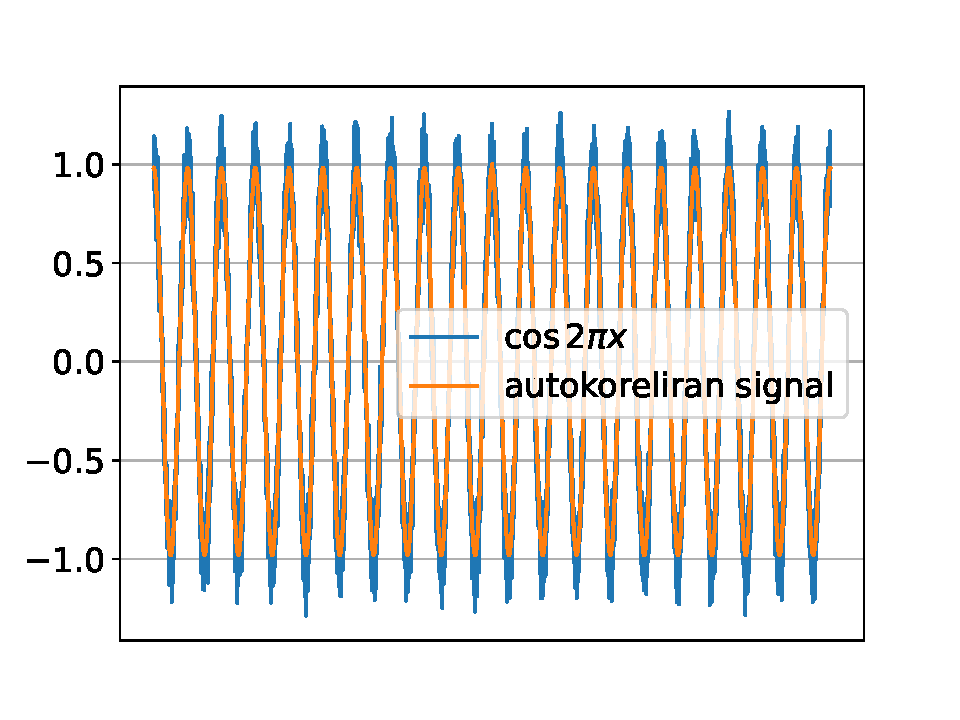
\includegraphics[width=\textwidth]{cosine.pdf}
    \end{minipage}%
    \hfill
    \begin{minipage}{0.5\textwidth}
        \centering
        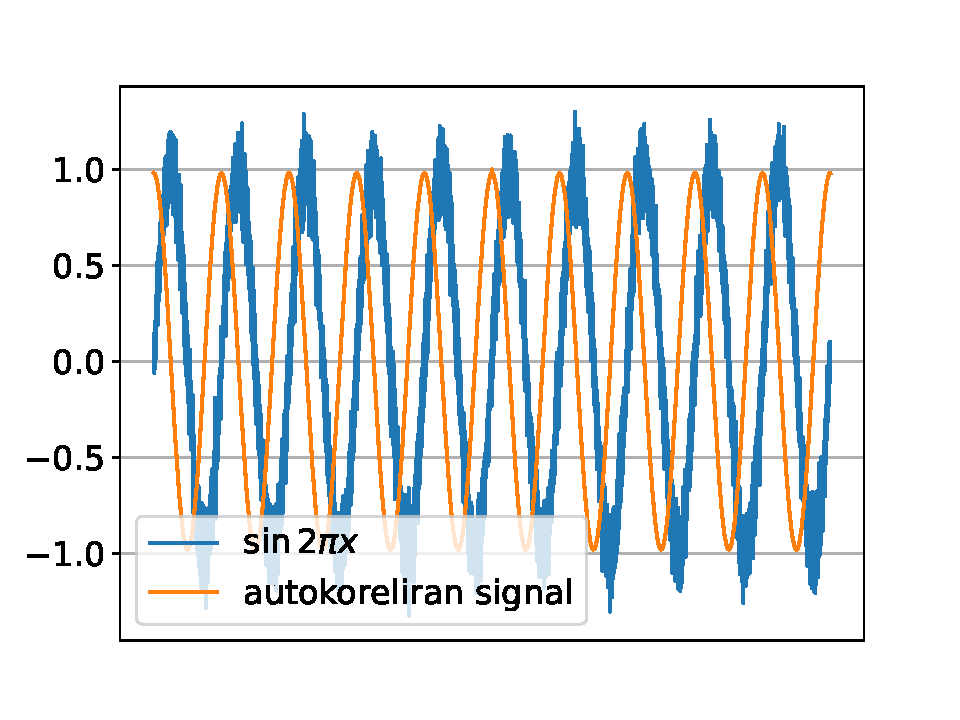
\includegraphics[width=\textwidth]{sine.pdf}
    \end{minipage}
	\caption{Korelacija sinusne in kosinusne funkcije}
\end{figure}
Pri zašumljenemu kosinusu, ki je soda funkcija opazimo, da se avtokorelacija funkcije lepo prilega. Pri sinusu pa so podatki rahlo zamaknjeni, saj je liha funkcija. Avtokorelacija pa nam vedno vrne sodo funkcijo in bi bilo potrebno za popolno prilagajanje še ročno dodati fazo.
\subsection{Sove}
Podana sta nam posnetka dveh sov. Poleg tega pa dobimo še 4 posnetke v katerih je zašumljena ena izmed prejšnjih sov. Za lažjo primerjavo bomo prvo imenovali Borut drugo pa Paul. Za začetek naredimo avtokorelacijo, kot nam diktirajo navodila. 
\begin{figure}[H]
    \centering
    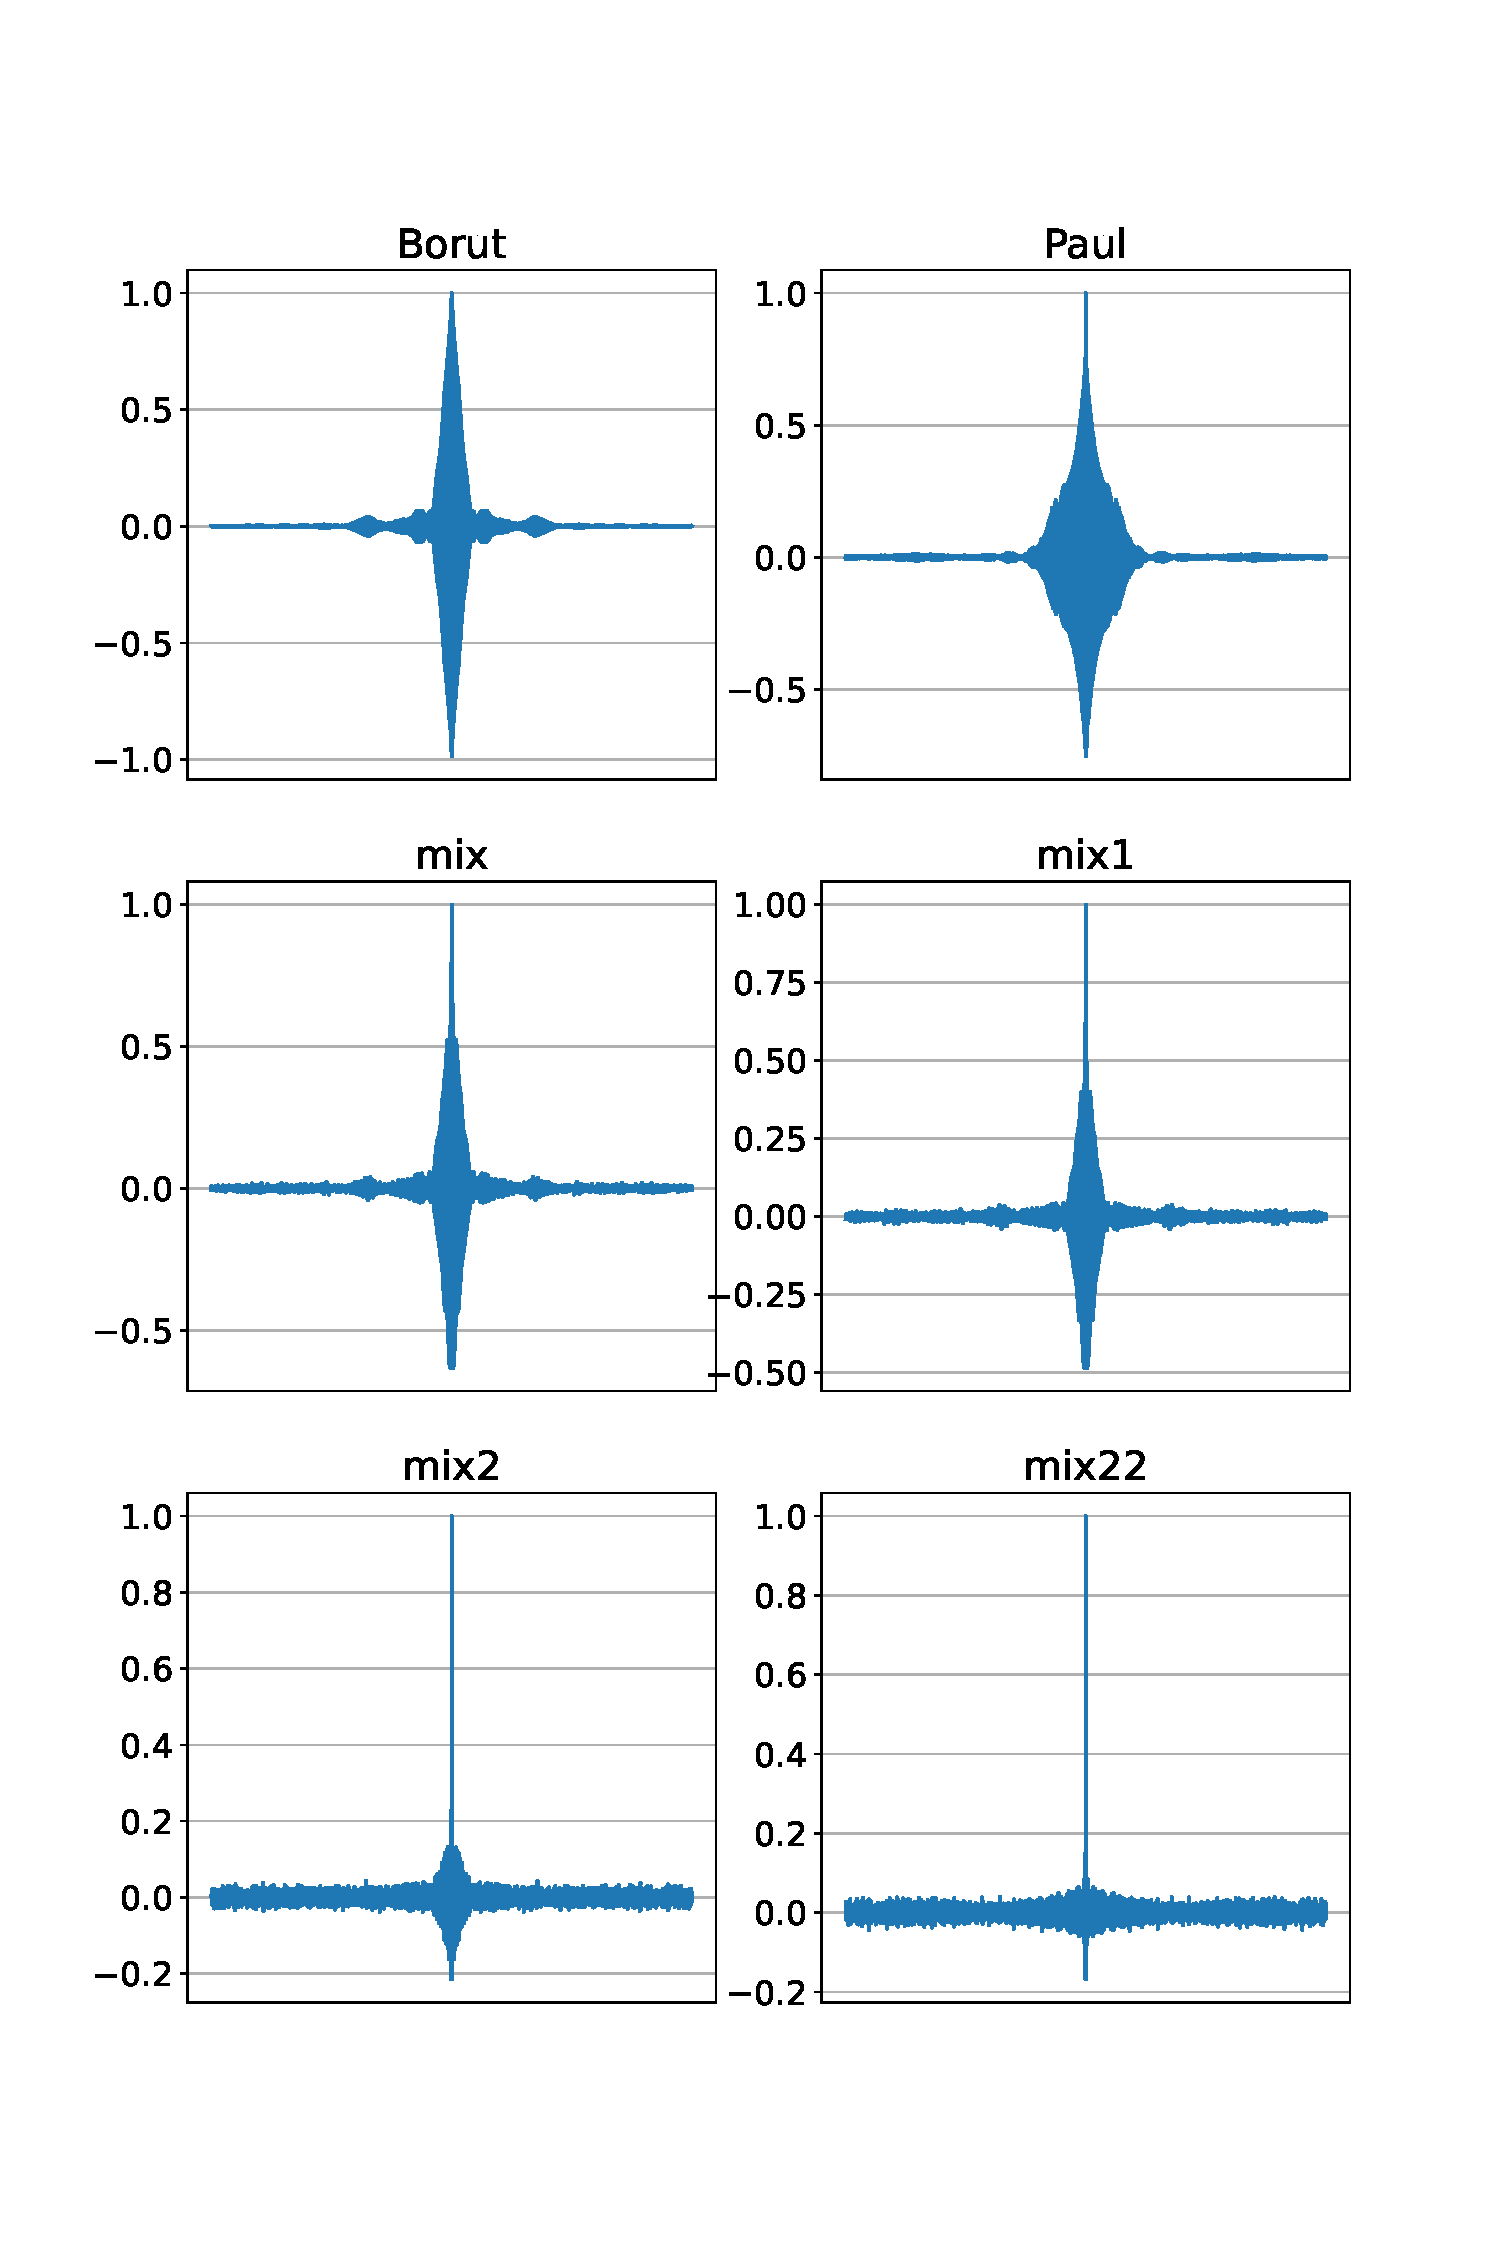
\includegraphics[width=0.8\textwidth]{autocor1.pdf}
	\caption{Avtokorelacija na vseh podanih posnetkih dveh sov}
    \label{fig:example}
\end{figure}
V prvi vrsti zgornjega grafa sta dva čista posnetka Boruta in Paula. V prvih dveh posnetkih s šumom lahko kar hitro opazimo, da je v obeh Borut. V tretjem pa nam ozkost signala tudi namiguje v to smer. V zadnjem primeru pa je signal praktično neopazen zato o njem ne moremo reči prav veliko. Prva intuitivna ideja kako bi lahko o zadnjih dveh signalih izvedeli več je, da avtokorelacijo ponovimo še enkrat.
\begin{figure}[H]
    \centering
    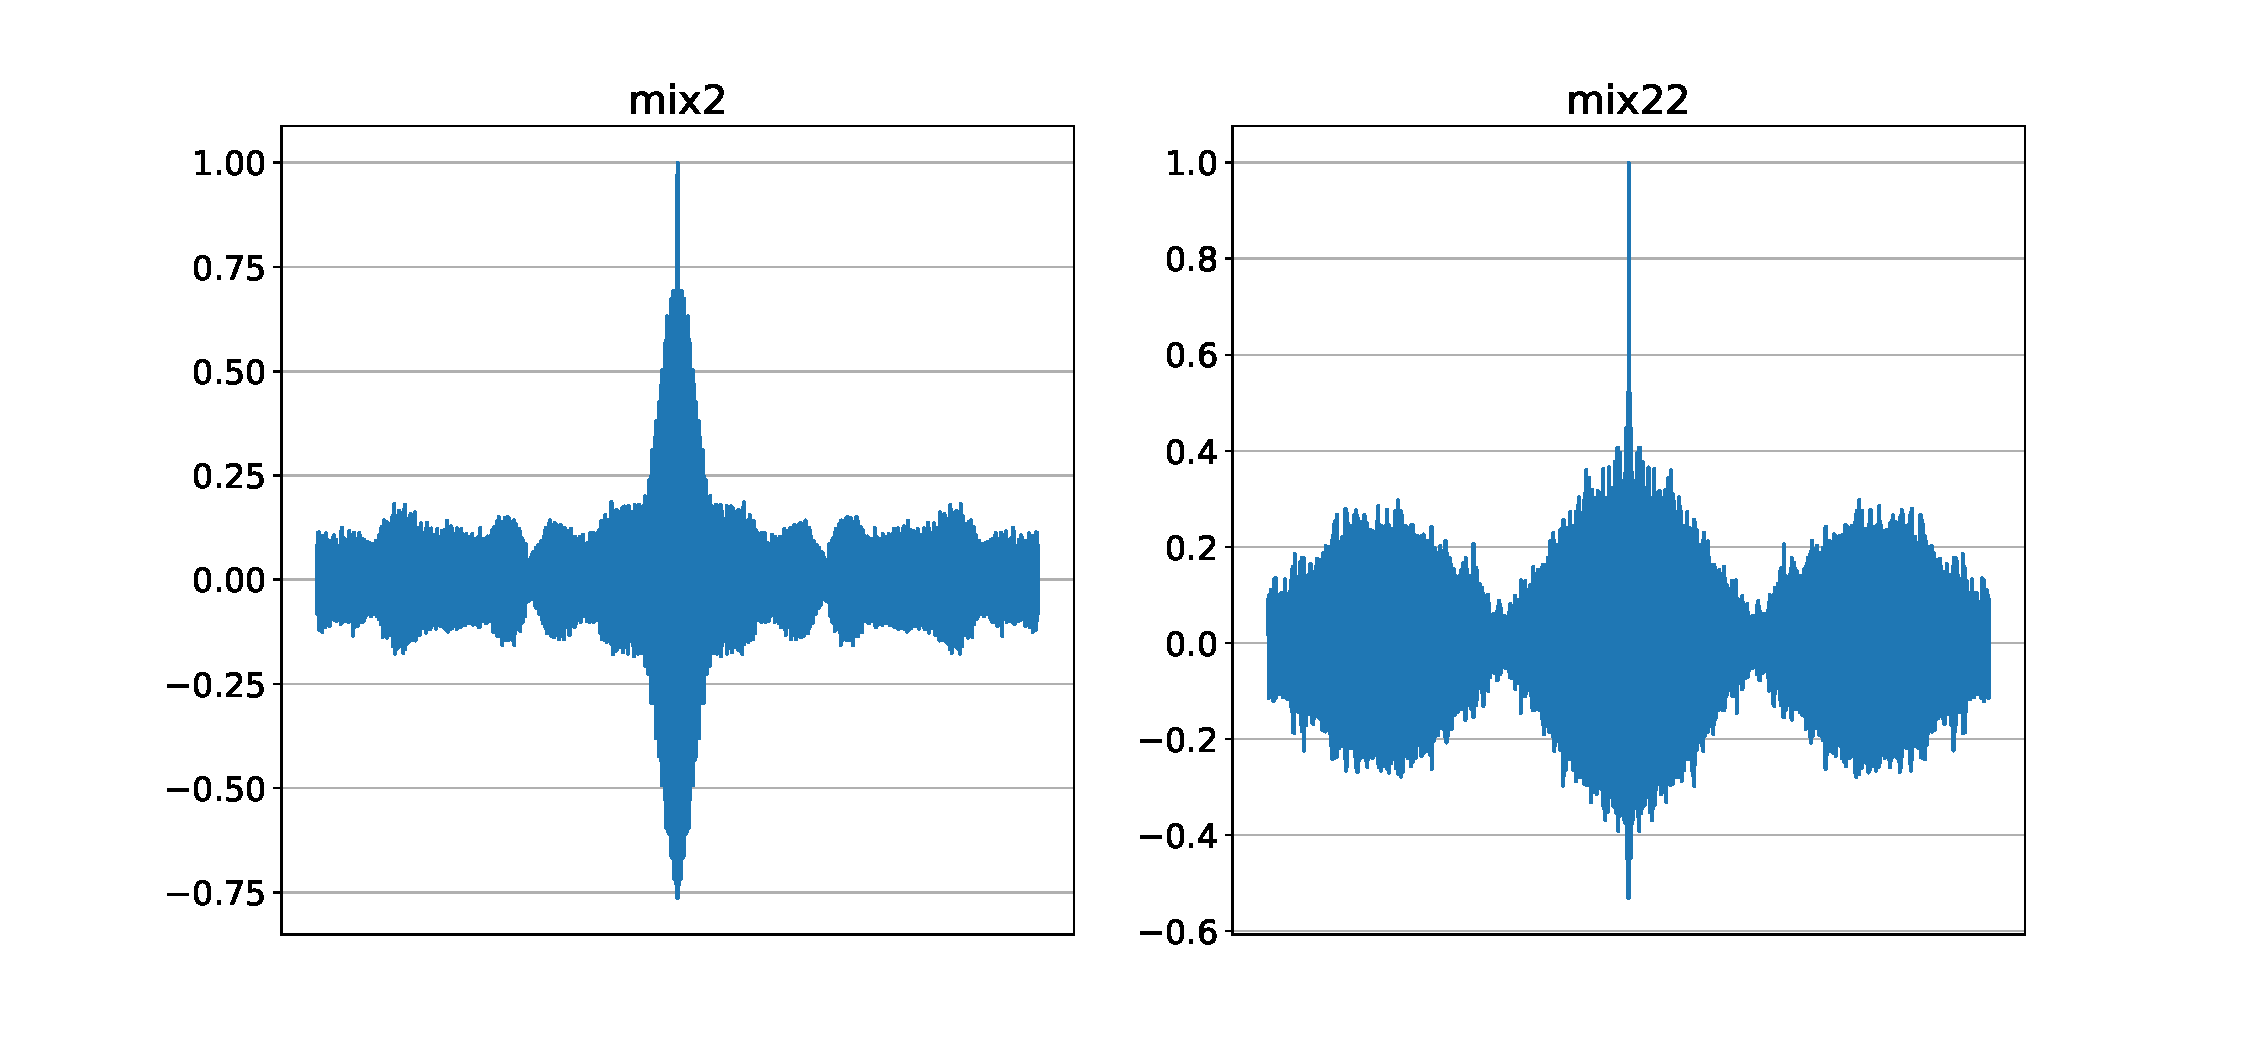
\includegraphics[width=0.8\textwidth]{autocor2.pdf}
	\caption{Dvojna avtokorelacija na zadnjih dveh posnetkih sov}
    \label{fig:example}
\end{figure}
Ponovitev avtokorelacije nam potrdi naše prejšnje ugibanje, da je tretji signal posnetek Boruta. Zadnji posnetek pa ima precej unikatno obliko glede na ostale. Zato očitno to ni pravi pristop pri zadnji sovi. Zato poskusimo namesto avtokorelacije uporabiti korelacijo s čistima signaloma obeh sov.
\begin{figure}[H]
    \centering
    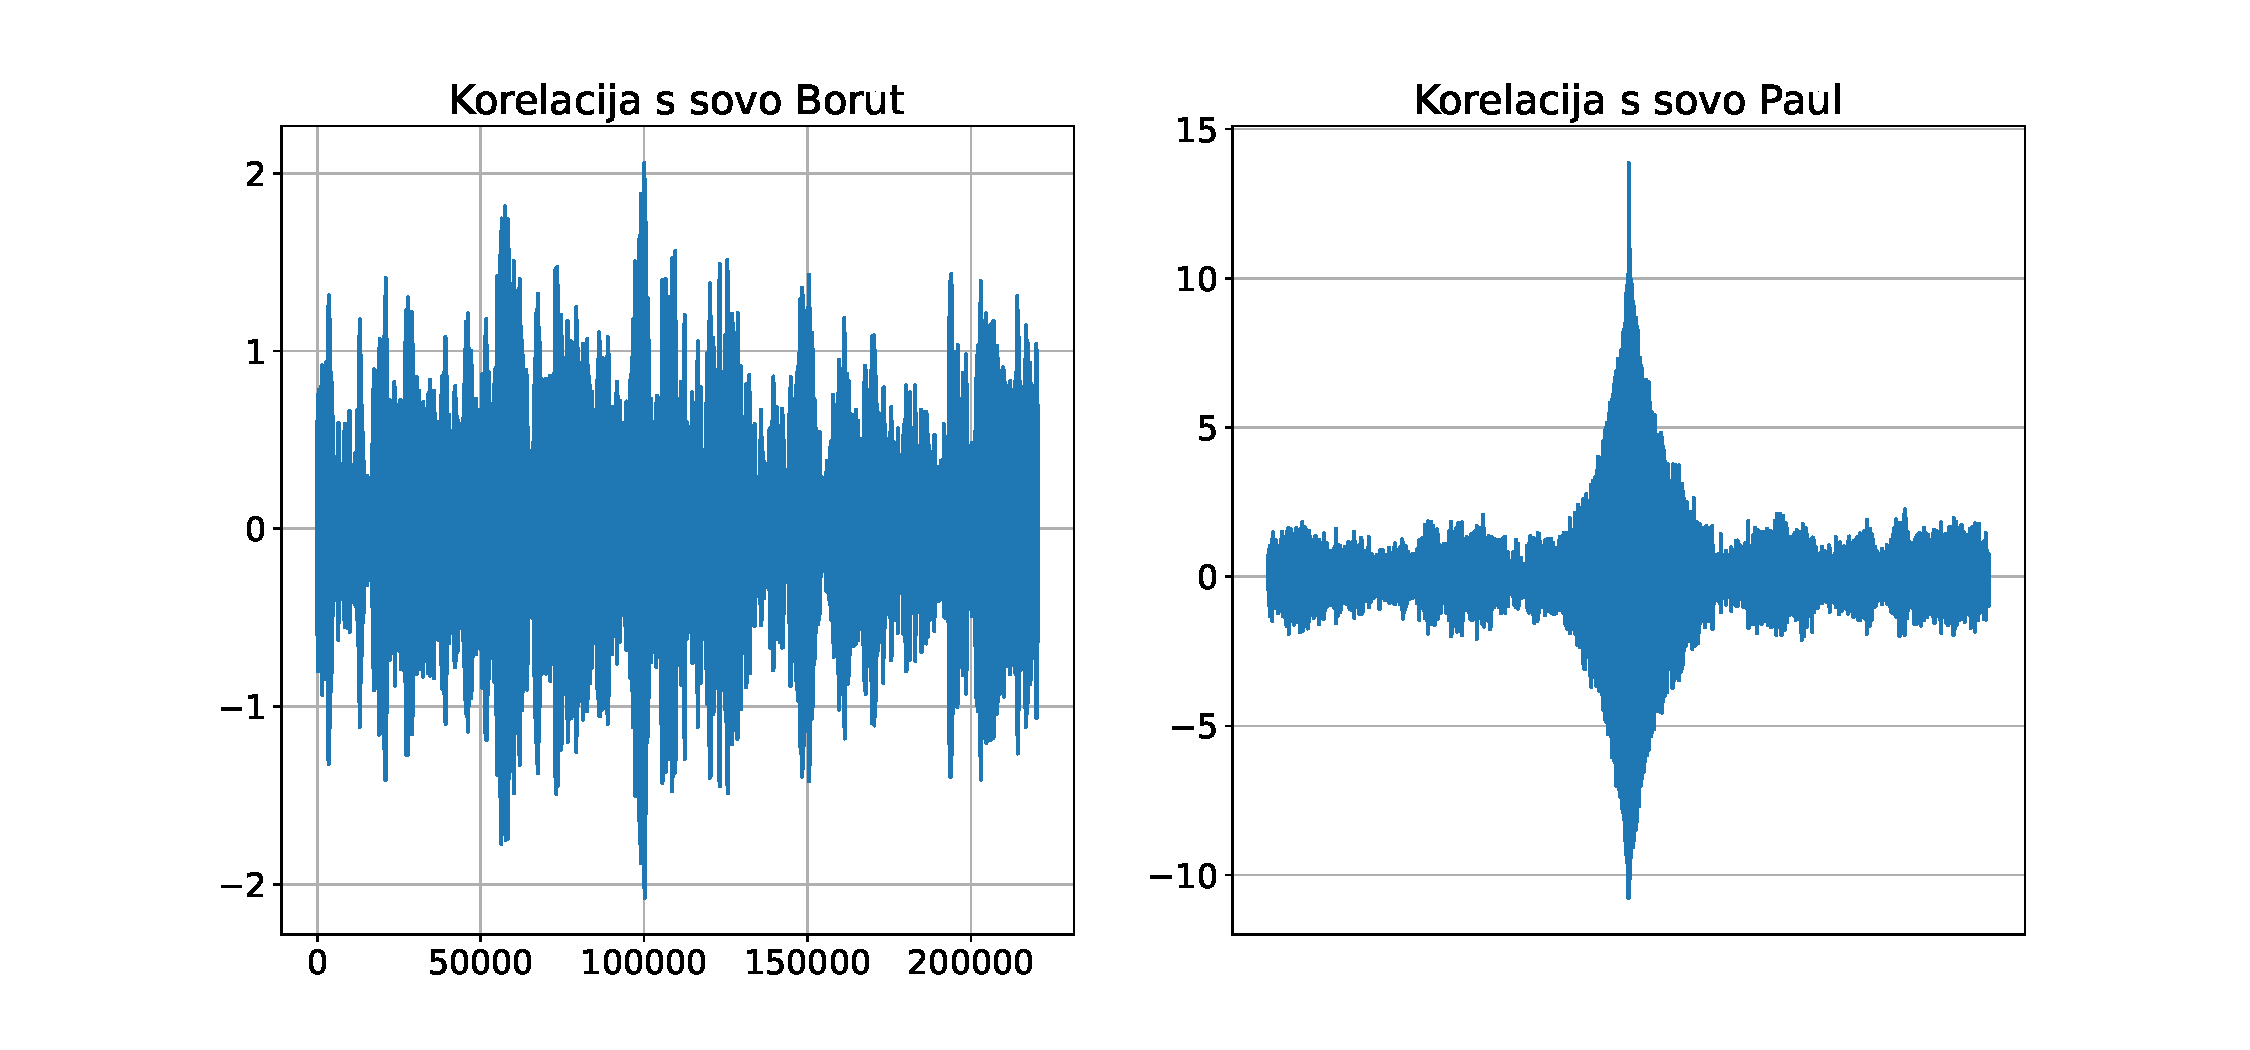
\includegraphics[width=0.8\textwidth]{autocorlast.pdf}
	\caption{Korelacija zadnjega posnetka s posnetkom Boruta in Paula}
    \label{fig:example}
\end{figure}
Tako nam korelacija pove, da je na zadnjem posnetku Paul. Če povzamemo naše ugotovitve smo ugotovili, da je na prvih treh zašumljenih posnetkih Borut na zadnjem pa Paul.
\subsection{Dodatna naloga}
Ob navodilu za dodatno nalogo sem se hitro spomnil na enega izmed mojih projektov, kjer sem iz vremenskih satelitov NOAA posnel signale slik Zemlje. Za obdelavo zvočnega signala bomo uporabili aplikacijo `noaa-apt image decoder`, ki je na voljo na internetu. Tako bomo najprej primerjali nastalo sliko pred našo obdelavo z avtokorelacijo in z obdelavo.  
\begin{figure}[H]
    \begin{minipage}{0.5\textwidth}
        \centering
        \includegraphics[width=\textwidth]{earth.png}
		\caption{Slika Zemlje iz prejetega signala}
    \end{minipage}%
    \hfill
    \begin{minipage}{0.45\textwidth}
        \centering
        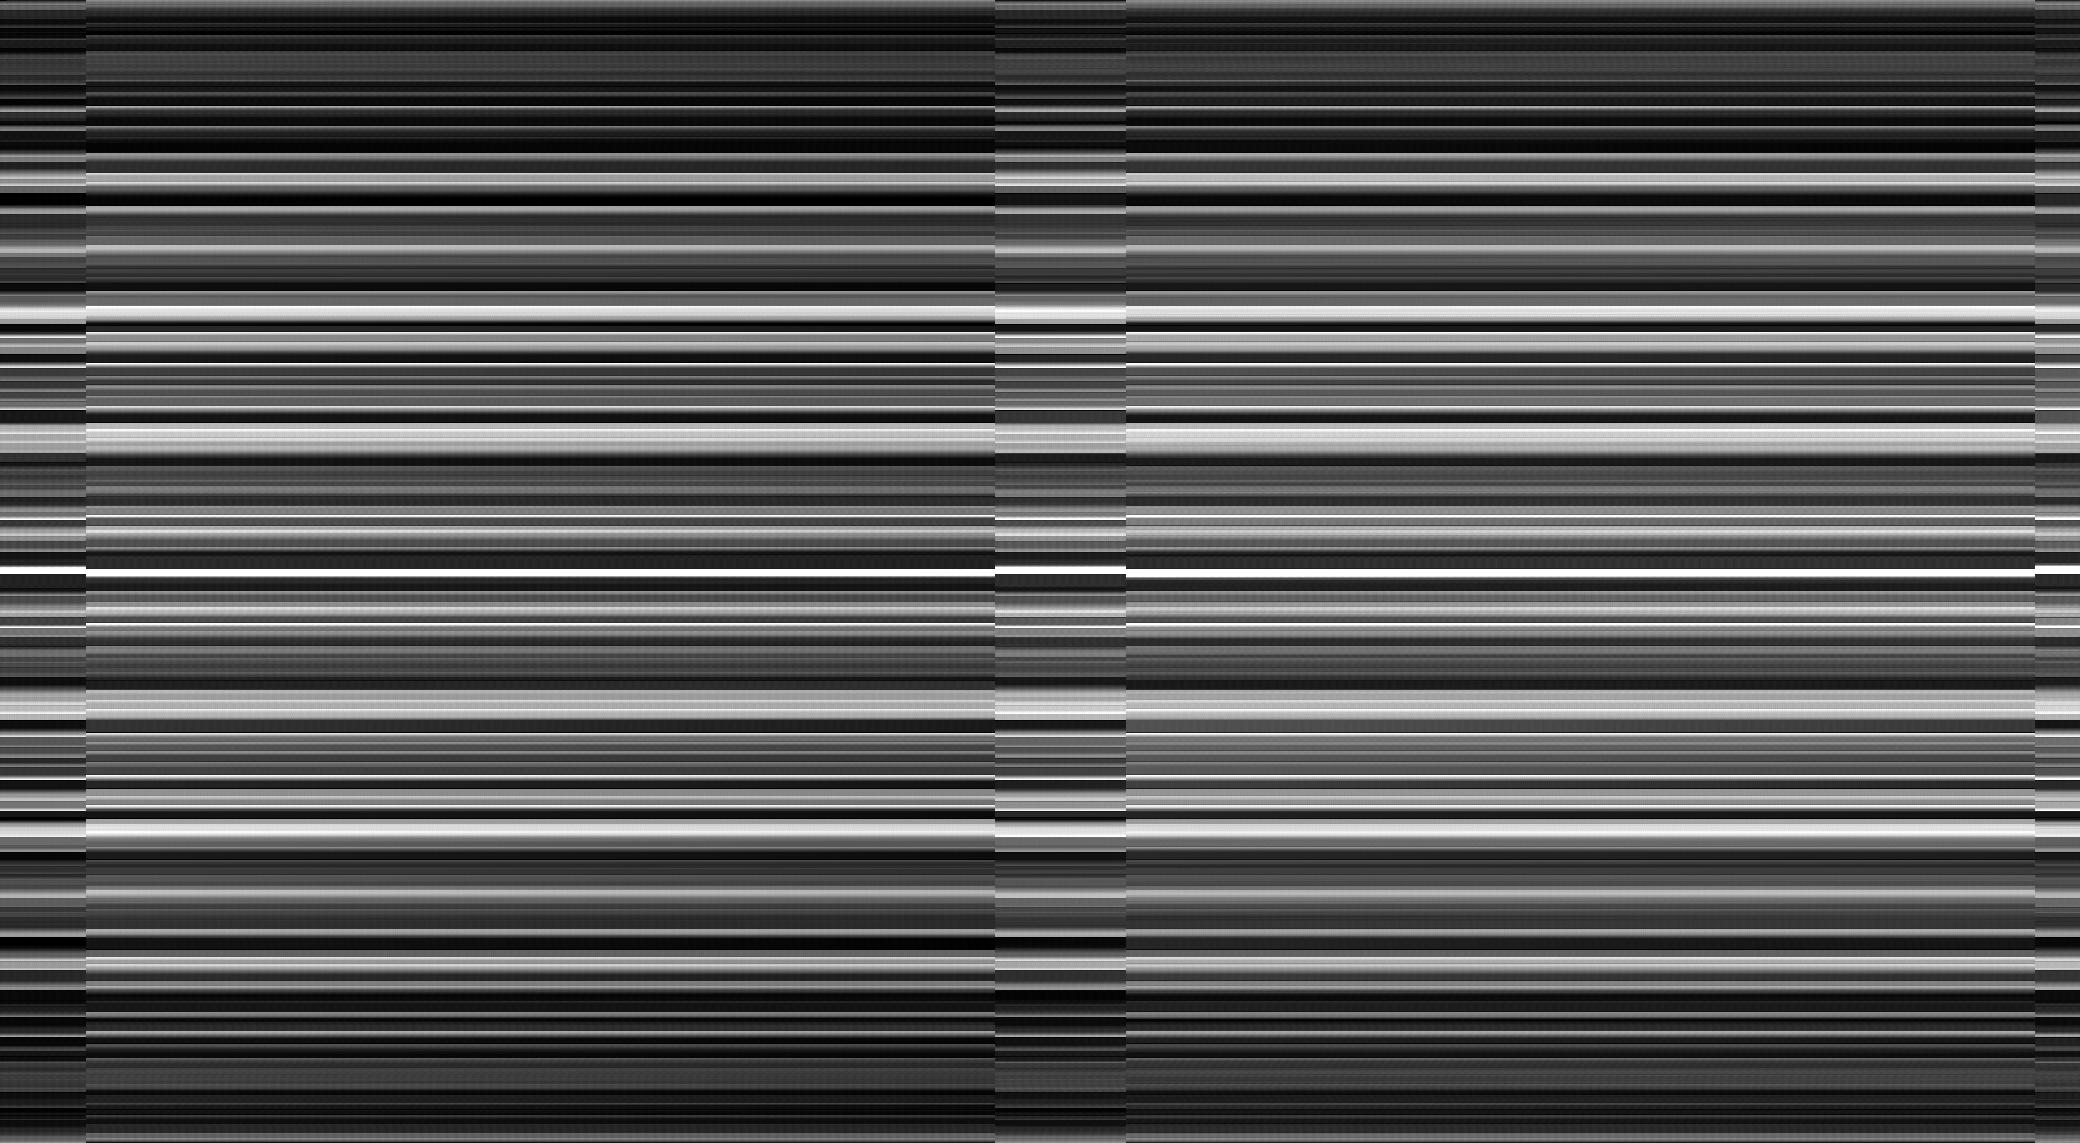
\includegraphics[width=\textwidth]{earthafter.png}
		\caption{Slika zemlje po obdelavi signala z avtokorelacijo}
    \end{minipage}
\end{figure}
Kar zelo hitro opazimo, da je avtokorelacija sliko naredila nerazpoznavno. Razloge za to lahko iščemo v dejstvu, da je signal z dejanskimi podatki zelo kompleksen in pri visokih frekvencah. Zato avtokorelacija težje izboljša signal.
\section{Zaključek}
Naloga nas je postavila pred zanimiv identificiranja sov in nam na preprost način pokazala uporabnost avtokorelacije pri razpozanavanju signalov. Za konec pa prilagam še \href{https://www.twobraids.com/2024/01/air-cannon.html}{povezavo do projekta o iskanju zračnega topa.}
\end{document}
